%%%%%%%%%%%%%%%%%%%%%%%%%%%%%%%%%%%%%%%%%%%%%%%%%%%%%%%%%%%%%%%%%%%%%%%%
%%%  THIS TEX FILE IS TO GENERATE PDF FILE FOR 
%%% 
%%%  COPYRIGHT (C) JIMMY LIN, 2013, UT AUSTIN
%%%%%%%%%%%%%%%%%%%%%%%%%%%%%%%%%%%%%%%%%%%%%%%%%%%%%%%%%%%%%%%%%%%%%%%%
\documentclass[11pt,a4paper]{article}
%%%%%%%%%%%%%%%%%%%%%%%%%%%%%%%%%%%%%%%%%%%%%%%%%%%%%%%%%%%%%%%%%%%%%%%%
%%%  PACKAGES USED IN THIS TEX SOURCE FILE
%%%%%%%%%%%%%%%%%%%%%%%%%%%%%%%%%%%%%%%%%%%%%%%%%%%%%%%%%%%%%%%%%%%%%%%%
\usepackage{geometry,amsthm,amsmath,graphicx,amssymb,fancyheadings}
\usepackage[]{mcode}
\usepackage[colorlinks,
            linkcolor=blue,
            anchorcolor=red,
            citecolor=green
            ]{hyperref}
% for my mac
\IfFileExists{/Users/JimmyLin/.latex/UTA_CS/JS.sty}{ 
    \usepackage{/Users/JimmyLin/.latex/UTA_CS/JS}
    \usepackage{/Users/JimmyLin/.latex/UTA_CS/JSASGN}
}{} 
% for UT's linux machine
\IfFileExists{/u/jimmylin/workspace/Configs/latex/UTA_CS/JS.sty}{
    \usepackage{/u/jimmylin/.latex/UTA_CS/JS} 
    \usepackage{/u/jimmylin/.latex/UTA_CS/JSASGN}
}{} 
%%%%%%%%%%%%%%%%%%%%%%%%%%%%%%%%%%%%%%%%%%%%%%%%%%%%%%%%%%%%%%%%%%%%%%%%
%%% MACROS CONTAINING THE FILE INFORMATION
%%%%%%%%%%%%%%%%%%%%%%%%%%%%%%%%%%%%%%%%%%%%%%%%%%%%%%%%%%%%%%%%%%%%%%%%
\renewcommand{\COURSE}{EE381V Large Scale Optimization}
\renewcommand{\LECTURER}{Sujay Sanghavi}
\renewcommand{\SECTION}{17350}
\renewcommand{\TASK}{Problem Set 4}
\renewcommand{\RELEASEDATE}{September 12, 2014}
\renewcommand{\DUEDATE}{September 18, 2014}
\renewcommand{\TIMECONSUME}{10 hours}
%%%%%%%%%%%%%%%%%%%%%%%%%%%%%%%%%%%%%%%%%%%%%%%%%%%%%%%%%%%%%%%%%%%%%%%%
%%% DOCUMENTATION STARTS FROM HERE 
%%%%%%%%%%%%%%%%%%%%%%%%%%%%%%%%%%%%%%%%%%%%%%%%%%%%%%%%%%%%%%%%%%%%%%%%
\begin{document}
%%%%%%%%%%%%%%%%%%%%%%%%%%%%%%%%%%%%%%%%%%%%%%%%%%%%%%%%%%%%%%%%%%%%%%%%
%% TITLE PAGE
%%%%%%%%%%%%%%%%%%%%%%%%%%%%%%%%%%%%%%%%%%%%%%%%%%%%%%%%%%%%%%%%%%%%%%%%
\begin{titlepage}
    \maketitle
\end{titlepage}
%%%%%%%%%%%%%%%%%%%%%%%%%%%%%%%%%%%%%%%%%%%%%%%%%%%%%%%%%%%%%%%%%%%%%%%%
%% CONTENT PAGE: TABLEOFCONTENTS, LISTOFTABLES, LIST OF FIGURES
%%%%%%%%%%%%%%%%%%%%%%%%%%%%%%%%%%%%%%%%%%%%%%%%%%%%%%%%%%%%%%%%%%%%%%%%
\renewcommand{\contentsname}{Table of Contents}
\begin{center} 
    \tableofcontents 
    %\listoftables 
    \listoffigures
\end{center}
\newpage
%%%%%%%%%%%%%%%%%%%%%%%%%%%%%%%%%%%%%%%%%%%%%%%%%%%%%%%%%%%%%%%%%%%%%%%%
%%% GENERAL DOCUMENTATION BEGINS 
%%%%%%%%%%%%%%%%%%%%%%%%%%%%%%%%%%%%%%%%%%%%%%%%%%%%%%%%%%%%%%%%%%%%%%%%

\section{Matlab and Computational Assignment}
\subsection{Conjugate Gradient Algorithm}
%\subsubsection{}
{\bf Command} to be executed in matlab:
\begin{verbatim}
  >> x_init = [1 1]'; alpha = 0.3; bta = 0.8;
  >> [x, iter, all_costs] = gd_btls(x_init, @func, @func_grad, alpha, bta);
\end{verbatim}
{\bf Dump}
\begin{verbatim}
  Iter: 1, Cost: 5.292007e+00, Conv_Rate: 0.106142, gamma: 0.800000
  Iter: 44, Cost: 2.559267e+00, Conv_Rate: 1.000000, gamma: 0.000000
  Convergence reached!
\end{verbatim}
{\bf Minima}
\begin{verbatim}
    x = [-0.3379, -0.0031], obj = 2.559267 
   \end{verbatim}
{\bf Plot}
\begin{figure}[h]
    \centering
   % 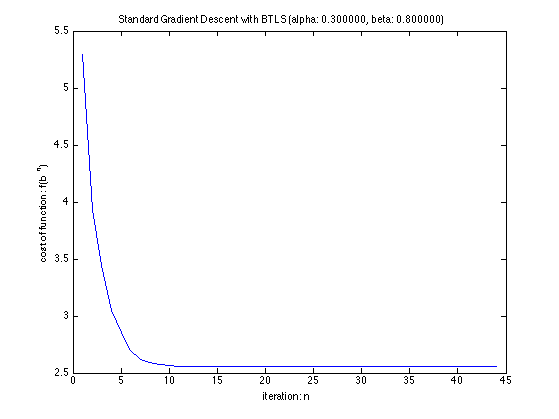
\includegraphics[width=5in,height=3in]{../ps2_matlab/1.png}
    \caption{Conjugate Gradient Algorithm}
\end{figure}

\newpage
\subsection{BFGS for Quadratic Problems}

\newpage
\subsection{Newton’s Method}

\newpage
\subsection{Central Path}


\newpage
\subsection{Larger Linear Program}

\newpage
\subsection{Gradient, Conjugate Gradient, Newton and BFGS}

\newpage
\section{Written Problems}
%\subsection{}

\newpage
\appendix
\section{Codes Printout}

\subsection{Eq. 20 and its gradient}
%\lstinputlisting{../ps4_matlab/func.m}

\newpage
\subsection{Standard Gradient Descent with BackTracking Line Search}
%\lstinputlisting{../ps4_matlab/gd_btls.m}

\newpage
\subsection{Steepest Descent with BackTracking Line Search}
%\lstinputlisting{../ps4_matlab/sd_btls.m}

\newpage
\subsection{Cyclic Coordinate Descent}
%\lstinputlisting{../ps4_matlab/ccd_btls.m}

\newpage
\subsection{Greedy Coordinate Descent}
%\lstinputlisting{../ps4_matlab/gcd_btls.m}
%%%%%%%%%%%%%%%%%%%%%%%%%%%%%%%%%%%%%%%%%%%%%%%%%%%%%%%%%%%%%%%%%%%%%%%%
%%% General Documentation ends
%%%%%%%%%%%%%%%%%%%%%%%%%%%%%%%%%%%%%%%%%%%%%%%%%%%%%%%%%%%%%%%%%%%%%%%%
\end{document}
